\chapter{Stand der Technik}


\section{Arten der Optimierung}
\label{sec:Sektion 31}

Die vorliegende Arbeit zielt auf die Bestimmung von energetischen Sanierungsmaßnahmen ab, welche für den deutschen Wohngebäudebestand möglichst kosteneffizient die C0\(_2\)-Emission reduziert.
Hierbei werden neben verschiedenen Möglichkeiten der Energiebereitstellung auch die energetische Qualität verschiedener Komponenten der Gebäudehülle betrachtet.
Dadurch ergibt sich eine hohe Anzahl an möglichen Kombinationsmöglichkeiten der Maßnahmen und Technologien.
Um aus dieser Komplexität ein Optimum zu bestimmen, ist es sinnvoll, ein rechnergestütztes Optimierungsprogramm als Werkzeug zu nutzen.

Eine Optimierung wird immer durch ein Ziel charakterisiert.
In einem mathematischen Sinne wird dieses als Zielfunktion beschrieben, welches es zu minimieren oder maximieren gilt.
Durch Rahmenbedingungen, auch Nebenbedingungen oder Restriktionen genannt, wird die Menge der zulässigen Lösungen beschränkt.
Dieser Lösungsraum wird durch Gleichungen oder Ungleichungen formuliert.
Sowohl die Zielfunktion als auch die Nebenbedingungen werden durch Variablen abgebildet.
Diese können anschaulich als Stellschrauben beschrieben werden.\cite{Schellong.2016}\\
Zusammenfassend kann eine Optimierung als das Lösen einer Zielfunktion in einem von Restriktionen beschränkten Lösungsraum durch eine Kombination von Variablen umschrieben werden. 

Im Folgenden stellt dieses Kapitel verschiedene Arten der Energiesystemoptimierung sowie diverse Beispiele an Optimierungsprogramme aus der Literatur vor, um letztlich das im Rahmen dieser Arbeit verwendete Programm in \ref{sec:Sektion 32} zu beschreiben.

Zur Einteilung von Optimierungsprogrammen existieren verschiedene Möglichkeiten.
Bei der Betrachtung der zu Grunde liegenden Variablen erhält man eine Unterteilung.
Hierbei werden die Programme in einer mathematischen Anschauung danach unterteilt, aus welchem Raum die Variablen entstammen.
So wird zwischen diskreten und kontinuierlichen Variablen unterschieden. 
Die diskreten entstammen dem Raum der ganzen Zahlen \(\mathbb{Z}\) und umfassen unter anderem Binärvariablen.
Letztere sind die Menge aus [0; 1] und werden im Rahmen der Energiesystemoptimierung oft als Option der Kaufentscheidung von Energiesystemen oder Schaltzustände der Anlagentechnik genutzt. 
Dabei beschreibt 0 einen ausgeschalteten, beziehungsweise nicht gekauften Zustand und 1 den eingeschalteten/gekauften.
Neben den diskreten Variablen werden auch kontinuierliche in Optimierungsprogrammen genutzt. 
Diese sind als reelle Zahlen \(\mathbb{R}\) definiert und beschreiben beispielsweise Kapazitäten, Heizbedarfe oder Wärmeverluste.
Werden in einem Programm diskrete und kontinuierliche Variablen gemischt, so spricht man von einer gemischt-ganzzahligen Optimierung. \cite{Schellong.2016}

Neben den Variablen stellt die Art der Funktionen eine weitere Unterscheidung der Optimierungsprogramme dar.
Bestehen die Restriktionen und die Zielfunktion eines Programmes einzig und allein aus linearen Zusammenhängen, so wird von einem linearen Programm (LP) gesprochen.
Dem gegenüber werden solche Optimierungen, welche auch Nichtlinearitäten abbilden, als nicht-lineare Programme (NLP) bezeichnet.
Oftmals findet man in der Realität nicht-lineare Zusammenhänge, welche mit NLP gut modelliert werden können.
Als ein Beispiel aus der Gebäudeenergiesystemoptimierung sei hier das Teillastverhalten von Wärmeerzeugern genannt.
Jedoch stellt das Lösen von nicht-linearen Gleichungen einen erhöhten Rechenaufwand dar, welcher mit einer deutlich längeren Rechendauer einhergeht.
Somit kann durch die Linearisierung von nicht-linearen Zusammenhängen Rechenzeit zu Kosten von Genauigkeit eingespart werden. 
Die gemischt-ganzzahlige lineare Optimierung wird aufgrund ihrer englischen Bezeichnung (\glqq Mixed Integer Linear Programing\grqq)\,mit MILP abgekürzt, die nicht-lineare analog mit MINLP. \cite{Samsatli.2018} 

In der Literatur werden verschiedene Ansätze und Modelle für die Optimierung von Energiesystemen verfolgt.
Diese werden durch die betrachtete Gebäude- oder Quartiersebene, der Zielfunktion, den zu Grunde liegenden Energiesystemen und der Betrachtung von Auslegungs- oder Betriebsoptimierung des Systems charakterisiert

Iturriaga et al. \cite{Iturriaga.2017} erarbeiten ein allgemeines Modell zur Auslegung von Energiesysteme auf Gebäudeebene. 
Dieses soll alle derzeit verfügbaren Technologien der Wärme-, Kälte- und Elektrizitätsbereitstellung abbilden können.
Hierzu werden die Anlagen unterteilt in solche, welche hohe, mittlere und niedrige Temperaturen erzeugen, Kältemaschinen und elektrische Module.
Thermische und elektrische Energie kann zwischen den jeweiligen Energiebereitstellungstechnologien ausgetauscht werden, um letztlich den Wärme-, Kälte- und Elektrizitätsbedarf des Gebäudes zu decken.
Weiterhin berücksichtigt das Modell neben der Energieerzeugung auch Speicher und Interaktionen mit anderen Gebäuden durch Nah-, Fernwärme- sowie Stromnetze.
Das Modell wird anhand eines Beispielgebäudes im nordspanischen Bilbao getestet.
Hierbei werden 13 verschiedenen Technologien der Wärme- und Elektrizitätserzeugung in Betracht gezogen.
Diese umfassen neben Organic-Rankine-, Gasturbinen- und Verbrennungsmotoren-Blockheizkraftwerke (BHKW) auch verschiedene solarthermische Anlagen (CPC, Vakuumröhrenkollektoren, Flachkollektoren), Biomasse-, Gas- und Brennwertkessel, Luft-Wasser-Wärmepumpen (WP) und diverse Photovoltaik-Anlagen (PV) (amorphe, mono- und polykristalline Solarmodule).
Die stückweise Linearisierung des nicht-linearen Teillastverhaltens der Anlagen führt zu rein linearen Gleichungen und somit zu einem MILP Problem.
Als Zielfunktion ist die Minimierung der annualisierten Kosten definiert. 
Diese setzen sich aus Investitionen, jährlichen variablen Kosten, Energiebezugskosten sowie Gewinnen aus dem Verkauf an überschüssiger Wärme, Kälte oder Elektrizität zusammen.
Als Restriktionen der Optimierung sind technologische Nebenbedingungen der Anlagentechnik, die Bedarfserfüllung des Gebäudes, gebäudespezifische Rahmenbedingungen sowie die möglichen Ausprägungen der Variablen aufgeführt.

In \cite{Pinzon.23.04.201726.04.2017} wird ein Modell von Pinzon et al. zur Optimierung der jährlichen Elektrizitätskosten unter Berücksichtigung der Behaglichkeit der Bewohner vorgestellt.
Die Berechnung dieser Kosten berücksichtigt den Strombedarf zu Heiz- oder Kühlzwecken, zur Beleuchtung sowie Ersparnisse aus PV.
Weiter existiert die Option erzeugten Strom, Wärme oder Kälte in einem Energiespeicher (ES) zu lagern.
Wie in Iturriaga et al. \cite{Iturriaga.2017} werden nicht-lineare Gleichungen durch stückweise Linearisierung in lineare gewandelt.
Dadurch handelt es sich bei dem Programm von Pinzon et al. um ein betriebsoptimierendes MILP Problem.
Als Zielfunktion ist die Minimierung des Strombedarfes und somit der Stromkosten beschrieben.
Der Bedarf setzt sich aus dem Verbrauch der zuvor genannten Komponenten zusammen.
Als Nebenbedingungen werden die Nutzung der PV-Anlagen, des ES, des Klimageräts und der Beleuchtung sowie die Einhaltung des thermischen Komforts definiert.
Bei letzterem werden auch die Wärmeträgheit des Luftvolumens im Raum, sowie der Wärmeverlust durch den Infiltrationsluftvolumenstrom, also durch Undichtheiten in der Gebäudehülle, berücksichtigt.

In Risbeck et al. \cite{Risbeck.2017} wird der optimale Betrieb von Lüftungssystemen zum Kühlen und Wärmen in kommerziellen Gebäuden, also Nichtwohngebäuden, untersucht.
Hierzu werden diskrete Variablen zum Modellieren des An- und Abschaltens der Komponenten sowie kontinuierliche zur Abbildung der Lasten und Speicherstände genutzt.
Als Zielfunktion werden minimale Betriebskosten bei Einhaltung des thermischen Komforts im Gebäude formuliert.
Auch Risbeck et al. wandeln nicht-lineare Geräteverhalten durch stückweise Linearisierung in lineare um und modellieren somit ein MILP.
Dadurch wird die Rechenzeit verkürzt und das Programm kann in Echtzeit auf Preisänderungen, Bedarfsschwankungen und Wetteränderungen eingehen.
Als Nebenbedingungen der Optimierungsaufgabe werden neben der Temperierung verschiedener Gebäudezonen auch die optimale Nutzung der zur Verfügung stehenden Speicher beachtet.

Zhu et al. stellen in \cite{Zhu.2019} eine multikriterielle Energsystemoptimierung vor.
Hierbei werden thermische und elektrische Speicher zur optimalen Kapazitätsauslegung untersucht und als übergeordnetes Modell definiert.
Weiter wird hierfür der Betrieb der Energieerzeuger optimiert, was das untergeordnete Modell umschreibt.
Zur Deckung des Wärme- und Elektrizitätsbedarfs werden eine Sole-WP, PV und Strombezug aus dem Netz modelliert.
Die Energiespeicherung erfolgt durch einen sensiblen Wasserspeicher und eine Batterie.
Ein Teil der nicht-linearen Gleichungen werden linearisiert. 
Da jedoch weiterhin nicht-lineare Zusammenhänge in dem Programm existieren, handelt es sich bei dem Modell um ein MINLP, welches Energiesysteme auf Gebäudeebene optimiert.
Als Zielfunktion des übergeordneten Modells wird die Minimierung der jährlichen Gesamtkosten festgelegt.
und als das der untergeordneten Optimierung die jährlichen Betriebskosten der Energieerzeuger.

Eine glechzeitige Betrachtung von Anlagentechnik und Gebäudehülle ist in Asadi et al. zu finden \cite{Asadi.2012}.
Hierbei handelt es sich zum einen um ein MINLP und zum anderen um eine multikriterielle Optimierung, bei welcher dem Programm mehrere Zielfunktionen übergeben werden.
Das Modell betrachtet neben Dämmarten und -stärke der Außenwand und des Dachs auch den Fenstertyp sowie Solarkollektoren. 
Hierzu wird für jedes Bauteil zwischen unterschiedlichen Sanierungsszenarien unterschieden.
Weiter wird der Energiebedarf des Gebäudes vereinfacht als Summe des Wärme-, Kälte- und Warmwasserbedarfes berechnet.
Ziel des Programmes ist die Bestimmung des kosten- und emissionsoptimalen Energiesystems.

In \cite{Wouters.2014} modellieren Wouters et al. Haushalte, die auf Quartiersebene thermische und elektrische Energie untereinander austauschen können.
An Anlagentechnik stehen Brennwertkessel, BHKWs, ES, PV-Anlagen und kleine Windkraftanlagen (WKA) zur Verfügung.
Als Zielfunktion ist die Minimierung der Annuität durch optimale Anlagenwahl, -auslegung und -betrieb definiert.
Das Programm wird nur mit linearen Gleichungen modelliert, sodass es sich um ein MILP handelt.
Weiter werden Einflüsse regulatorischer Maßnahmen untersucht und darauf aufbauend zwei Standorte mit ähnlichen klimatischen Bedingungen in Griechenland und Australien miteinander verglichen.

Das Optimierungsmodell von Harb et al. \cite{Harb.2016} bestimmt die optimale Anlagenauswahl zur Wärmeerzeugung von Einzelwohngebäuden oder Quartieren.
Es werden Mikro-BHKWs, Wärmepumpen, Elektroheizstäbe, PV, thermische Speicher, Kessel sowie Nahwärmenetze in Betracht gezogen.
Das MILP von Harb et al. benennt als Ziel die Minimierung der jährlichen Kosten, welche sich aus annualisierten Investitionen, Bedarfskosten sowie den variablen Kosten zusammensetzen.
Das Modell von Harb et al. zeichnet aus, dass die Einspeisevergütung von PV-Strom sowie die Förderung von BHKW produzierter Elektrizität in die wirtschaftliche Betrachtung mit einfließen.

Eine simultane Betrachtung der Energieerzeuger und der Gebäudehülle liegt in Schütz et al. \cite{Schutz.2017} vor.
Hier werden sowohl der Betrieb als auch die Auslegung des Gebäudeenergiesystems optimiert.
Das Programm berücksichtigt neben Energieerzeugern und -speichern wie Kessel, BHKW, Elektroheizstäbe (EHS), WP, Solarthermie, PV und ES auch energetische Ertüchtigungen der Außenwand, der Fenster, des Daches und der Bodenplatte.
Als Optimierungsziel kann zwischen Jahres-Kosten- und Emissionsoptimierung gewählt werden.
Weiter besteht die Möglichkeit einer Pareto-Optimierung, bei welcher die nicht gewählte Zielfunktion als Nebenbedingung das Modell beschränkt.

In Tabelle \ref{tab: Tabelle311} sind die zuvor vorgestellten Programme der Energiesystemoptimierung mitsamt ihren charakteristischen Eigenschaften aufgeführt.

\begin{table}[H] \centering
\begin{tabular}{|l|l|l|l|l|}
\hline
\rowcolor[HTML]{C0C0C0} 
Autor & \begin{tabular}[c]{@{}l@{}}Art der\\ Optimierung \end{tabular} & \begin{tabular}[c]{@{}l@{}}Ebene/ \\ Betrachtung \end{tabular} & Energiesysteme & \begin{tabular}[c]{@{}l@{}}Zielfunktion\\ (Minimierung von...)\end{tabular} \\ \hline
Iturriaga et al. & MILP & \begin{tabular}[c]{@{}l@{}}Gebäude\\ Auslegung\end{tabular} & XXXX & Jährliche Kosten \\ \hline
\rowcolor[HTML]{EFEFEF} 
Pinzon et al. & MILP & \begin{tabular}[c]{@{}l@{}}Gebäude\\ Betrieb\end{tabular} & PV, ES,Klimageräte & \begin{tabular}[c]{@{}l@{}}Jährliche Elektri-\\ zitätskosten\end{tabular} \\ \hline
Risbeck et al. & MILP & \begin{tabular}[c]{@{}l@{}}Gebäude\\ Betrieb\end{tabular} & Lüftungssysteme & \begin{tabular}[c]{@{}l@{}}Jährliche Betriebs-\\ kosten\end{tabular} \\ \hline
\rowcolor[HTML]{EFEFEF} 
Zhu et al. & MINLP & \begin{tabular}[c]{@{}l@{}}Gebäude\\ Auslegung und\\ Betrieb\end{tabular} & PV, WP, ES & \begin{tabular}[c]{@{}l@{}}Jährliche Betriebs-\\ kosten\end{tabular} \\ \hline
Asadi et al. & MINLP & \begin{tabular}[c]{@{}l@{}}Gebäude\\ Auslegung\end{tabular} & \begin{tabular}[c]{@{}l@{}}Sanierung von Wand, \\ Dach, Fenster/\\ Solarkollektoren\end{tabular} & \begin{tabular}[c]{@{}l@{}}Kosten und\\ Emissionen\end{tabular} \\ \hline
\rowcolor[HTML]{EFEFEF} 
Wouters et al. & MILP & \begin{tabular}[c]{@{}l@{}}Quartier\\ Auslegung und \\ Betrieb\end{tabular} & \begin{tabular}[c]{@{}l@{}}Kessel, BHKW, ES, \\ PV, WKA\end{tabular} & Jährliche Kosten \\ \hline
Harb et al. & MILP & \begin{tabular}[c]{@{}l@{}}Gebäude/\\ Quartier\\Auslegung\end{tabular} & \begin{tabular}[c]{@{}l@{}}Mikro-BHKW, WP,\\ EHS, PV, \\ thermische ES, Kessel, \\ Nahwärmenetz\end{tabular} & Jährliche Kosten \\ \hline
\rowcolor[HTML]{EFEFEF} 
Schütz et al. & MILP & \begin{tabular}[c]{@{}l@{}}Gebäude\\ Auslegung und \\ Betrieb\end{tabular} & \begin{tabular}[c]{@{}l@{}}Kessel, BHKW, \\ EHS, WP, Solarthermie, \\ PV, ES/\\ Sanierung von Wand, \\ Dach, Fenster, Boden\end{tabular} & \begin{tabular}[c]{@{}l@{}}Kosten und/\\ oder Emissionen\end{tabular} \\ \hline
\end{tabular}
\caption{Übersicht diverser Ansätze der Energiesystemoptimierung in der Literatur}
\label{tab: Tabelle311}
\end{table}


\section{Referenzmodell als Grundlage dieser Arbeit}
\label{sec:Sektion 32}

Im Rahmen der vorliegenden Arbeit wird ein Programm zur Kosten- oder Emissionsoptimierung von Gebäudeenergiesystemen erweitert.
Neben einer Auswahl an Anlagentechniken zur Energiebereitstellung stehen Maßnahmen zur energetischen Ertüchtigung der Gebäudehülle zur Verfügung. 
Hierbei werden ähnlich wie bei Asadi et al. \cite{Asadi.2012} und Schütz et al. \cite{Schutz.2017} Außenwände, Fenster und Dächer sowie zusätzlich die Grundplatte betrachtet.
Die dem Programm zu Grunde liegende Anlagentechnik ist in Tabelle \ref{tab: Tabelle321} aufgeführt.
Die Entscheidung für verschiedene Anlagen oder Maßnahmen an der Hülle erfolgt durch diskrete Binärvariablen, wohingegen die Auslegung und der Betrieb durch kontinuierliche Variablen modelliert wird.
Wie in Iturriaga et al. \cite{Iturriaga.2017}, Pinzon et al. \cite{Pinzon.23.04.201726.04.2017} und Risbeck et al. \cite{Risbeck.2017} erfolgt eine Linearisierung der nicht-linearen Gleichungen, sodass es sich um ein MILP handelt.
Die Zielfunktion der Optimierung kann entweder zur Minimierung der annualisierten Kosten oder CO\(_2\)-Emissionen gesetzt werden.
Des weiteren besteht die Möglichkeit eine Pareto-Optimierung durchzuführen, bei welcher ein Gebäudeenergiesystem unter Berücksichtigung der Kosten- und Emissionsoptimierung ermittelt wird.

Das zu berechnende Gebäude wird eingangs anhand verschiedener Parameter durch den Nutzer beschrieben.
Hierzu zählen unter anderem das Baujahr, die Gebäudegröße und der Standort.
Anhand dieser Eingabewert greift das Programm auf hinterlegte Daten zu, um weitere Parameter in das Programm mit aufzunehmen.
Weiter werden die 365 Tage eines Jahres in einigen wenigen, repräsentativen Typtagen zusammengefasst, um somit die Komplexität des Problems zu reduzieren.
Bei dem eigentlichen Optimierungsprozess wird ein Gleichungssystem basierend auf den zuvor gewählten und eingelesenen Parametern zur Minimierung der Zielfunktion gelöst.
Nach der Optimierung gibt das Programm Daten zu dem gewählten Energiesystem, den Kosten und den Emission aus, die dann vom Nutzer ausgewertet werden.
In Abbildung \ref{fig: Abbildung321} ist der Programmablauf schematisch skizziert.

\begin{figure}[H]
	\centering
		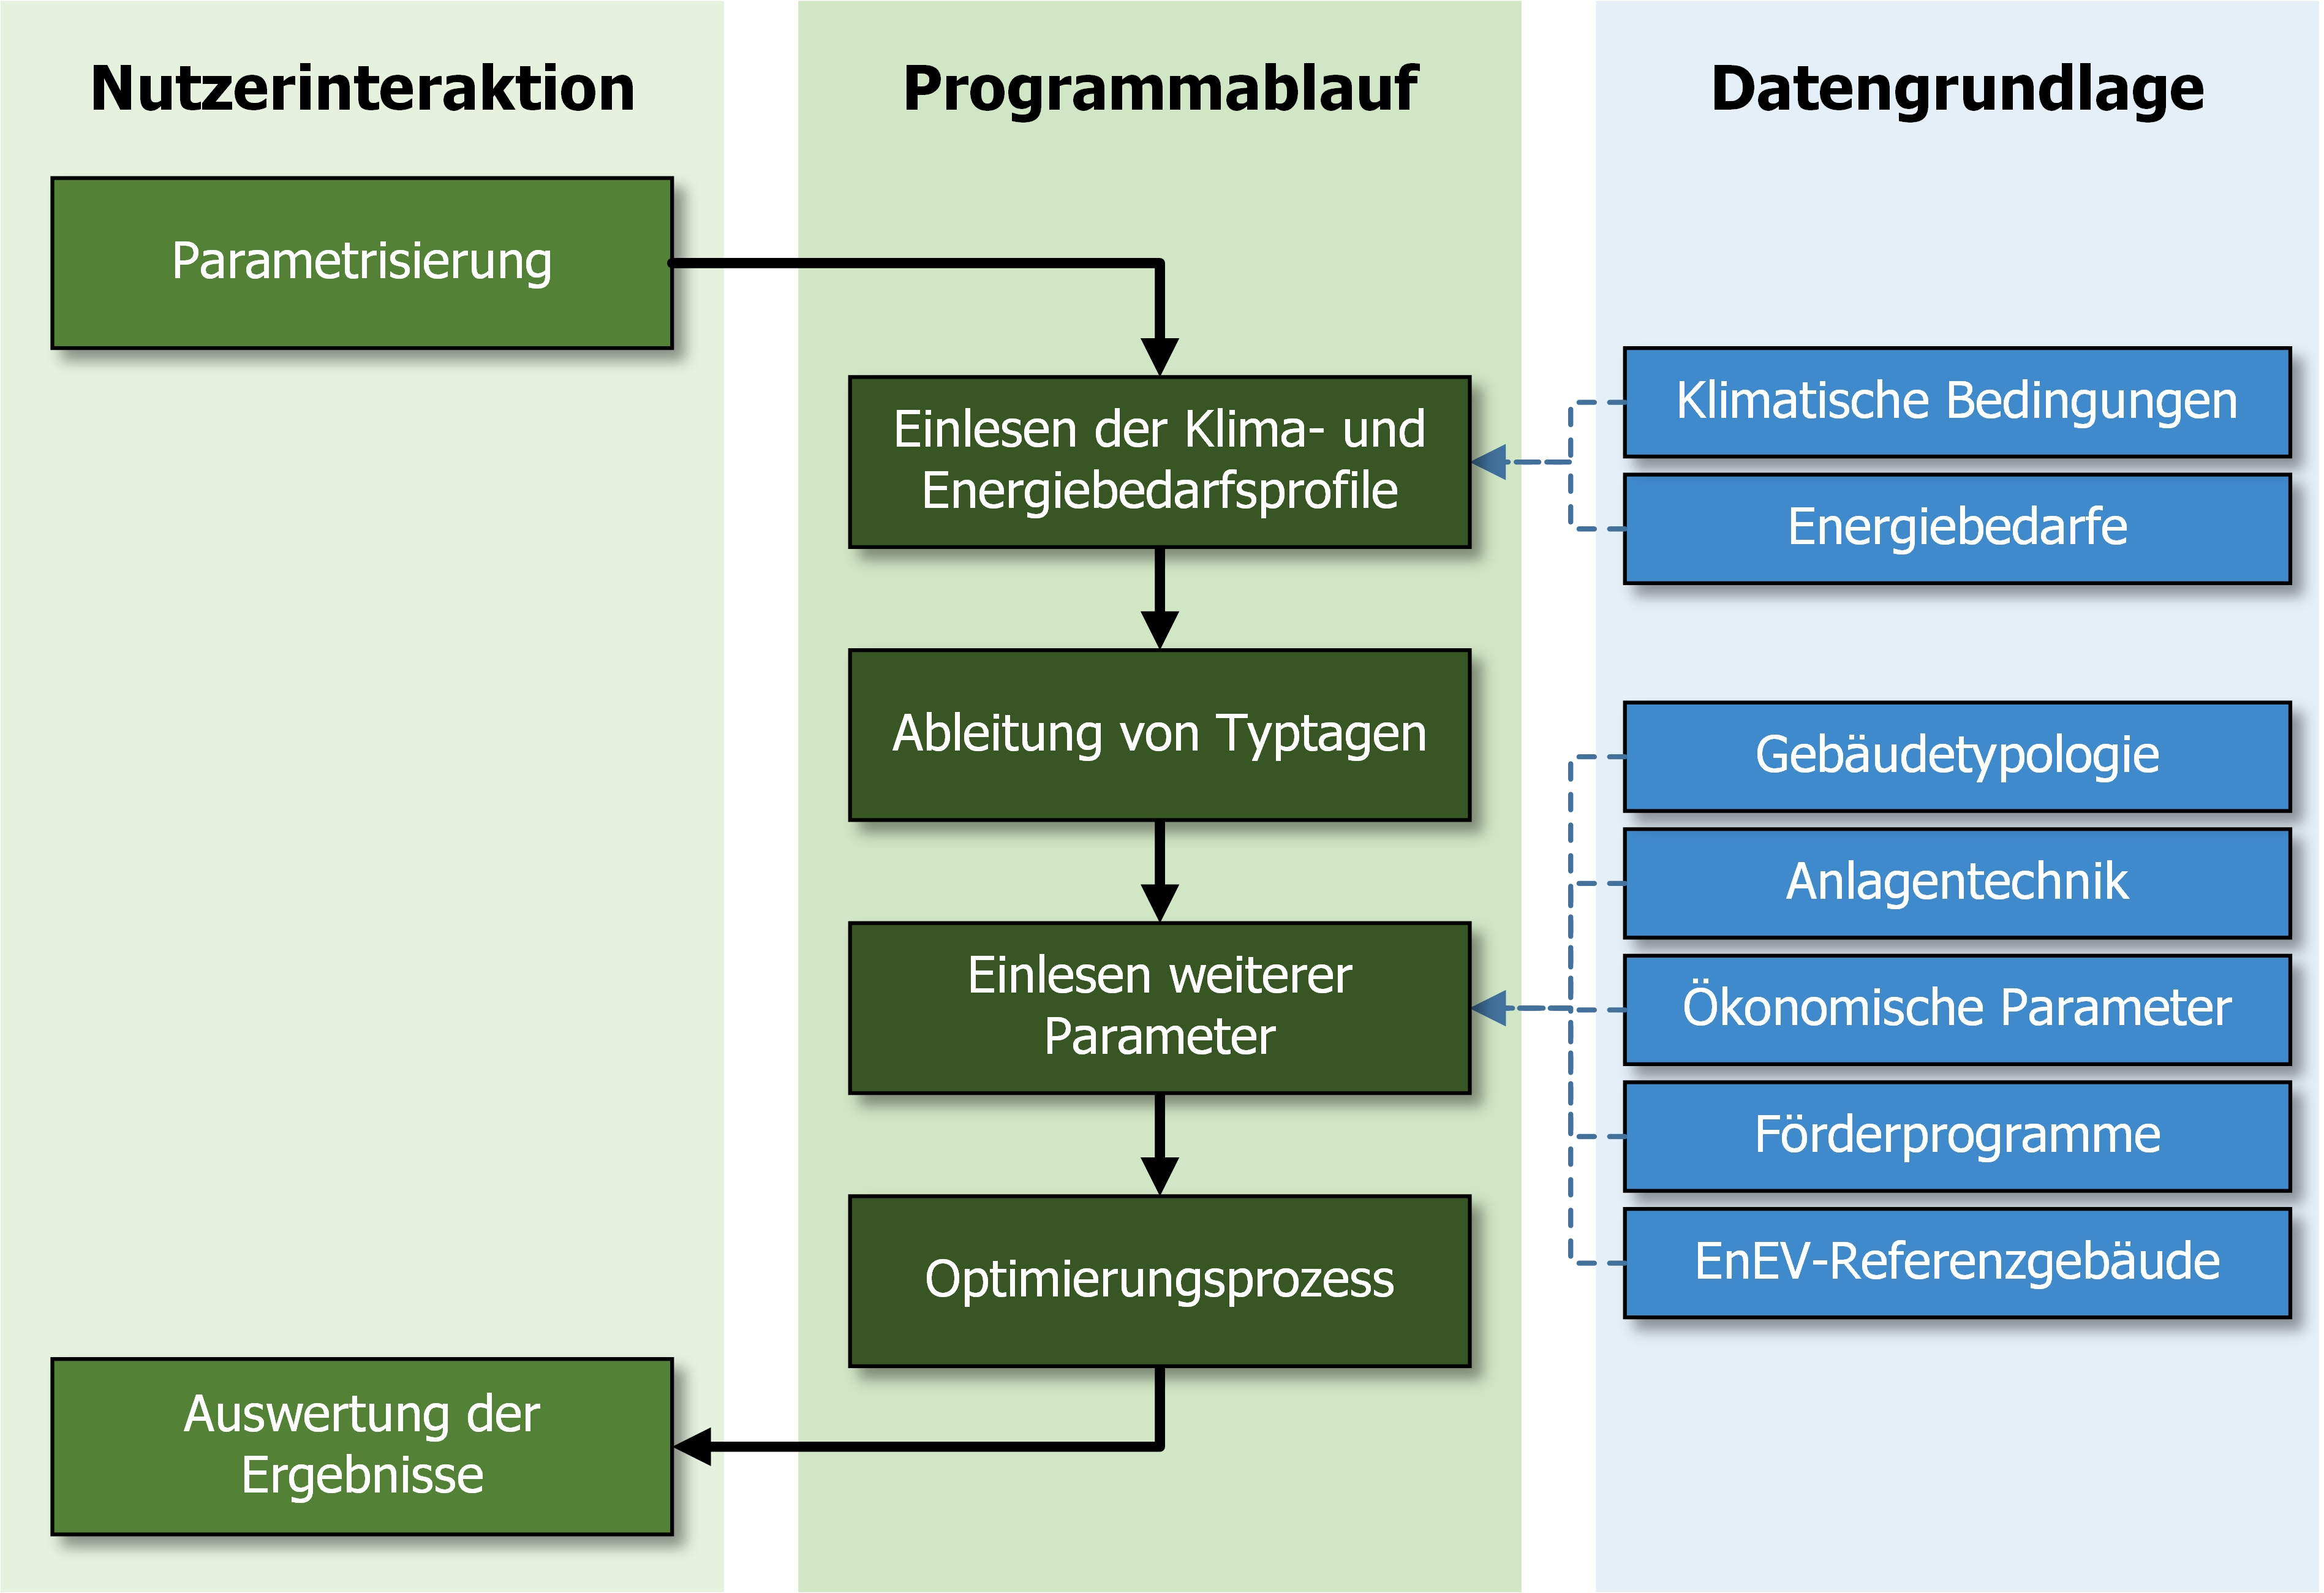
\includegraphics{Pictures/ProzessOptiProgramm.jpg}
	\caption{Schematischer Ablauf des Optimierungsprogrammes}
	\label{fig: Abbildung321} 
\end{figure}

Zunächst erfolgt die Parametrisierung des Gebäudes durch den Nutzer.
Hier werden Gebäudetyp, -alter und -lage sowie Wohnungsanzahl, Wohnfläche je Wohnung, Haushaltsgröße und qualitative Angaben zum Strom- und Trinkwarmwasserbedarfs definiert.
In Bezug auf den Gebäudetyp stehen die TABULA-Klassen Einfamilien-, Reihen-, Mehrfamilienhaus und Apartment-Block zur Wahl.
Auch die Baualtersklassen basieren auf TABULA-Unterteilungen und gliedern sich in 12 Klassen im Zeitraum von 1860 bis 2010.
Bei der Gebäudelage stehen dem Nutzer 15 verschiedene Standorte aus verschiedenen Klimaregionen Deutschlands zur Auswahl.
Eine Übersicht über die möglichen Ausprägungen der Inputparameter Gebäudealter und -lage ist Tabelle \ref{tab: TabelleA3} zu entnehmen. \cite{Loga.102012}

Wie in Abbildung \ref{fig: Abbildung321} dargestellt, startet in einem nächsten Schritt der Programmablauf mit dem Einlesen der Klima- und Energiebedarfsprofile.
Auf Basis der übergebenen Angaben wird auf eine Datengrundlage zurückgegriffen.
So werden anhand des Gebäudestandortes entsprechend jährliche Klimaprofile genutzt.
Diese entsprechen dem Testreferenzjahr des Deutschen Wetterdienstes, welches für den Betrachtungszeitraum von 1981 bis 2010 einen repräsentativen Witterungsverlauf beschreibt \cite{try}.
Neben einem Umgebungstemperaturverlauf liefern die Profile solare Einstrahlungen und sind stündlich, also in 8760 Zeitpunkte, aufgeteilt.
Weiter werden Strom- und Trinkwarmwasserbedarfsprofile sowie Profile der internen Gewinne eingelesen.
Im Falle der Einfamilien- und Reihenhäuser hängen diese von der Haushaltsgröße ab und bei den Mehrfamilienhäusern sowie Apartment-Blocks von der Wohnungsanzahl.
Außerdem bedingen die Angaben zur Höhe des Strom- und Trinkwarmwasserbedarfes die Auswahl der Profile.
Die eingelesenen Verläufe basieren auf stochastischen erzeugten Profilen des deutschen Stromspiegels und bilden Grundlasten sowie Lastspitzen ab \cite{stromspiegel}.
Wie bei den Klimaprofilen sind auch diese als stündliche Werte über ein Jahr aufgetragen.

Da eine Optimierung über jede Stunde eines Jahres mit einem großen Rechenaufwand einhergeht, erfolgt anhand der eingelesenen Profile eine Ableitung von Typtagen.
An Tagen mit vergleichbaren Witterungsverläufen ähneln sich die Energiebedarfsprofile, sodass diese im Rahmen des Programmes mit Hilfe eines Clusteringvorgangs zusammengefasst werden \cite{Dubielzig.2007}.
Um einerseits saisonale Effekte abzubilden und aussagekräftige Ergebnisse zu erhalten und andererseits die Rechenzeit des Programmes zu verkürzen, werden die 8760 Stunden eines Jahres in 8 Typtagen mit 192 Zeitpunkten zusammengefasst.
Diese besitzen wiederum Gewichtungen, welche in Summe 365 Tage und somit ein Jahr ergeben.

Neben den bereits erläuterten Klima- und Energiebedarfsprofilen wird als nächster Vorgang des Programmablaufes weitere Parameter eingelesen.
So werden für die Bauteile der Gebäudehülle U-Werte für drei Sanierungsszenarien in das Modell mit aufgenommen.
Bei diesen handelt es sich um den Standard-Zustand des parametrisierten Gebäudes im Bestand (\glqq standard \grqq), einer Aufrüstung auf den Standard nach EnEV 2014 (\glqq retrofit\grqq) und einer energetischen Nachrüstung nach heutigem Passivhaus-Standard (\glqq advanced retrofit \grqq) \cite{.2015}.
Zudem werden Faktoren zur Dimensionierung der Fenster-, Dach-, Boden- und Außenwandfläche eingelesen.\\
Schließlich werden auch ökonomische Faktoren zur Bestimmung des Preises einer Sanierungsmaßnahme in das Programm mit aufgenommen. 
Hierbei werden die Investitionen der Gebäudehüllenbestandteile als lineare Funktion ausgedrückt.
Außer bei den Fenstern berechnen sich diese Kosten anhand der zusätzlichen Dämmdicke im Zuge des Sanierungsszenario.
Im Falle der Verglasung wird die lineare Funktion anstelle der Dämmstärke in Abhängigkeit der Verbesserung des U-Wertes aufgestellt.
Die Werte für den y-Achsenabschnitt und die Steigung der linearen Funktionen für die einzelnen Bauteile basieren auf Berechnungen des IWU \cite{Hinz.10.08.2015} und sind in Tabelle \ref{tab: TabelleA4} aufgeführt.
Zusätzlich sind in dieser Tabelle Angaben zu der Nutzungsdauer der Komponenten zu finden, welche aus derselben Quelle entstammen.
Diese werden für die Berechnung der annualisierten Kosten benötigt.\\
Mit den bisher beschriebenen Daten lassen sich die Bedarfe des Gebäudes bestimmen.
Zur Deckung dieser werden verschiedene Energieerzeuger und -speicher zu dem Modell hinzugefügt.
Die Dimensionierung der jeweiligen Technologien erfolgt kontinuierlich.
Um die Investition der Anlagen zu berechnen, existieren Installationskosten mit einer Unterscheidung zwischen Einfamilien- oder Mehrfamilienhaus.
Zudem werden die Steigung und der y-Achsenabschnitt einer linearen Funktion zur Preiskalkulation an das Programm übergeben oder anhand von empirischen Herstellerangaben generiert.
Tabelle \ref{tab: Tabelle321} führt die verschiedenen Technologien, welche im Modell Beachtung finden, auf.

Weiter werden betriebswirtschaftliche Parameter eingelesen.
Hierbei werden neben allgemeinen Faktoren wie dem Betrachtungszeitraum, der Mehrwertsteuer, dem internen Zinssatz und der Inflationsrate auch energieträgerspezifische Kennwerte übergeben.
Bei letzteren handelt es sich zum einen um Preisänderungsfaktoren, welche zukünftige Preisänderungen der Energieträger abbilden und zum anderen um Einspeisevergütung von PV- oder BHKW-Strom und um die Energiesteuer.
In Tabelle \ref{tab: TabelleA6} sind die Parameter mit ihren jeweiligen Werten aufgeführt.\\
Außerdem werden Daten zur Modellierung von Förderprogrammen, welche die Verbesserung des Gebäudeenergiesystems subventionieren, mitaufgenommen.
Die Fördergelder beeinflussen die Wirtschaftlichkeit verschiedener Technologien und energetischen Sanierungsmaßnahmen.
Daher werden die leistungsabhängigen Förderhöhen mit in das Modell aufgenommen.
Ferner gibt es für alle Programme Bedingungen, welche für eine Auszahlung erfüllt seien müssen und monetäre Grenzen, in denen sich die Fördersumme minimal und maximal bewegt.
Einen Überblick über die Förderkonditionen und -grenzen werden in Tabelle XXXX dargelegt.\\
Um die Förderungen im Rahmen des KfW-Effizienzhaus-Programms zu erhalten, wird die Sanierungsmaßnahme mit einem EnEV-Referenzgebäude verglichen.
Das Referenzgebäude wird mit derselben Geometrie wie die des parametrisierten Gebäudes ausgeführt, die Gebäudehülle besitzt allerdings eine energetische Qualität nach EnEV-Vorgaben.
Die U-Werte der jeweiligen Bauteile nach EnEV sind in Tabelle \ref{tab: Tabelle322} aufgeführt.

\begin{table}[H]\centering
\begin{tabular}{|l|c|}
\hline
\rowcolor[HTML]{C0C0C0} 
Bauteil & U-Werte {[}\(\frac{\text{W}}{m^2 \cdot K}\){]} \\ \hline
Außenwand & 0,28 \\ \hline
\rowcolor[HTML]{EFEFEF} 
Boden & 0,35 \\ \hline
Dach & 0,20 \\ \hline
\rowcolor[HTML]{EFEFEF} 
Fenster & 1,30 \\ \hline
\end{tabular}
\caption{U-Werte der Gebäudehülle für ein EnEV-Referenzgebäude nach EnEV 2009.}
\label{tab: Tabelle322}
\end{table}

Wie aus dem schematischen Ablauf in Abbildung \ref{fig: Abbildung321} zu erkennen ist, folgt nach dem Einlesen aller zuvor erläuterten Parameter der eigentliche Optimierungsprozess.
Als Zielfunktion des Optimierungsprogrammes kann zwischen der Minimierung der annualisierten Kosten oder der CO\(_2\)-Emissionen ausgewählt werden.
Die Kosten setzten sich zusammen aus Investitionen durch die Anschaffung der Anlagentechnik und Ertüchtigung der Gebäudehülle (\(C_{Inv}\)), den Wartungs- und Instandhaltungskosten der Anlagen (\(C_{Var}\)), den Kosten aus dem Bedarf an Elektrizität und Brennstoffen (\(C_{Bedarf}\)), den Fixkosten durch Strom- und Gasbezug (\(C_{Fix}\)) sowie den Gewinnen aus dem Verkauf von Strom (\(R_{Erlös}\)) und die Zuschüsse aus Förderprogrammen (\(R_{Subv}\)).
\begin{equation}
\label{eq:Gleichung321}
C_{total} = \sum C_{Inv} + \sum C_{Var} + \sum C_{Bedarf} + \sum C_{Fix} - \sum R_{Erlös} - \sum R_{Subv}  
\end{equation}
Die Berechnung der Investitionen unterscheidet sich leicht zwischen Energieerzeugern und Hüllensanierung.
Es sei zu erwähnen, dass das Standard-Szenario den Bestandszustand beschreibt und somit nicht mit Kosten verbunden ist.
Letztlich wird in allen Fällen eine totale Investitionssumme berechnet und unter Beachtung der jeweiligen Nutzungsdauer, dem internen Zinssatz und der Inflationsrate annualisiert.
Wie in Tabelle \ref{tab: Tabelle321} zu sehen, unterscheiden sich die Nutzungsdauern der Technologien und der Sanierungsszenarien der Gebäudehülle.
Übersteigt die Nutzungsdauer der Komponente den Betrachtungszeitraum der Kalkulation, wird ein Restwert gebildet und dieser annualisiert.
Im Falle einer geringeren Nutzungsdauer als dem Betrachtungszeitraum berechnet das Programm eine Ersatzinvestition.
Somit ergeben sich auf Basis der unterschiedlichen Nutzungsdauern für keine Technologie oder Sanierungsmaßnahme einen Vorteil gegenüber einer Alternativen.\\
Die betriebsgebundenen Kosten für Wartung und Instandhaltung werden anteilig aus den Investitionen bestimmt und mit einem Faktor zur Inflationsbereinigung multipliziert.\\
Zur Bestimmung der bedarfsspezifischen Kosten wird die Summe aus verschiedenen Energiequellen gebildet. Jeder Summand besteht hierfür aus dem Bedarf des Energieträgers multipliziert mit den leistungsspezifischen Kosten, dem Preisänderungsfaktor der Bezugsgröße und dem Faktor zur Annualisierung der Kosten. 
Eine Ausnahme bilden die BHKWs, da bei diesen der Gaspreis um die Energiesteuer reduziert wird.
Dies ist eine Folge der Förderung durch das KWK-Gesetz.\\
Im Falle der Fixkosten liest das Programm Grundpreise für die Nutzung von Gas und Strom ein.
Für Erdgas betragen diese 138 \(\frac{\text{\euro}}{\text{a}}\) und für den Strombezug 73 \(\frac{\text{\euro}}{\text{a}}\). \\

\begin{table}[H]\centering
\begin{tabular}{|l|c|l|c|}
\hline
\rowcolor[HTML]{C0C0C0} 
\multicolumn{1}{l|}{\cellcolor[HTML]{C0C0C0}\begin{tabular}[c]{@{}l@{}}Technologie\\ Sanierungsmaßnahme\end{tabular}} & \multicolumn{1}{l|}{\cellcolor[HTML]{C0C0C0}\begin{tabular}[c]{@{}l@{}}Nutzungsdauer\\ in Jahren\end{tabular}} & \multicolumn{1}{l|}{\cellcolor[HTML]{C0C0C0}\begin{tabular}[c]{@{}l@{}}Technologie\\ Sanierungsmaßnahme\end{tabular}} & \multicolumn{1}{l|}{\cellcolor[HTML]{C0C0C0}\begin{tabular}[c]{@{}l@{}}Nutzungsdauer\\ in Jahren\end{tabular}} \\ \hline
\rowcolor[HTML]{EFEFEF} 
Brennwertkessel & 20 & Solarthermie & 20 \\ \hline
Luft-Wärmepumpe & 18 & PV & 20 \\ \hline
\rowcolor[HTML]{EFEFEF} 
Sole-Wärmepumpe & 20 & Thermischer Speicher & 20 \\ \hline
Pelletkessel & 20 & Batteriespeicher & 15 \\ \hline
\rowcolor[HTML]{EFEFEF} 
BHKW & 15 & Elektroheizstab & 20 \\ 
\hline \hline
Außenwand & 50 & Dach & 50 \\ \hline
\rowcolor[HTML]{EFEFEF}
Fenster & 50 & Bodenplatte & 50\\ \hline
\end{tabular}
\caption{Anlagentechnik und Maßnahmen der energetischen Ertüchtigung der Gebäudehülle sowie deren Nutzungsdauer im Optimierungsmodell}
\label{tab: Tabelle321}
\end{table}

Die Emission kann als Summe der CO\(_2\)-Freisetzung beschrieben werden, die durch den Bedarf an Brennstoffen entstehen.
Somit setzt sich die Berechnung der Emission aus der Verbrennung von Holz-Pellets (\(E_{Pellet}\)), Gas (\(E_{Gas}\)) und dem Emissionswert des Stromes aus Netzbezug (\(E_{Netz}\)) zusammen.
\begin{equation}
\label{eq:Gleichung322}
E_{total} = E_{Pellet} + E_{Gas} + E_{Netz}
\end{equation}
Die jeweiligen Summanden ergeben sich als Produkt aus dem Bedarf der Bezugsgröße und der leistungsspezifischen Emission der Emissionsquelle.
In Tabelle \ref{tab: Tabelle321} sind die Werte für die Energiequellen Holz-Pellets, Gas und Strom aufgeführt.

\begin{table}[H]\centering
\begin{tabular}{|l|c|}
\hline
\rowcolor[HTML]{C0C0C0} 
Energiequelle & \begin{tabular}[c]{@{}c@{}}CO\(_2\)-Emission\\ in {[}\(\frac{kg_{CO_2}}{kWh}\){]}\end{tabular} \\ \hline
\rowcolor[HTML]{EFEFEF} 
Holz-Pellets & 0,025 \\ 
\hline
Gas & 0,25 \\ 
\hline
\rowcolor[HTML]{EFEFEF} 
Strom & 0,566 \\ 
\hline
\end{tabular}
\caption{Leistungsspezifische Emission der Energieträger \cite{InstitutfurTechnischeGebaudeausrustungDresden.2017}}
\label{tab: Tabelle321}
\end{table}

Die Kombinationsmöglichkeiten zur Erfüllung der Zielfunktionen wird durch den Lösungsraum, welcher durch Restriktionen definiert wird, beschränkt.
So wird beispielsweise die Anzahl der PV-Module durch die zur Verfügung stehende Dachfläche limitiert.
Eine zentrale Nebenbedingung stellt die Berechnung der Heizlast dar.
Diese beschreibt die Wärmemenge, welche durch die Anlagentechnik bereitgestellt werden muss, um das Gebäude auf die Innentemperatur in Höhe von 20\,°C zu heizen.
Als Berechnungsgrundlage dient die DIN V 4108.
Diese definiert den Jahres-Heizenergiebedarf (Q) als Summe des Jahres-Heizwärmebedarfs (Q\(_h\), des Jahreswärmebedarfs zur Warmwasseraufbereitung (Q\(_W\) und den Wärmeverlusten der Anlagentechnik zur Wärme- und Warmwasserbereitstellung (Q\(_t\) abzüglich der Energiemenge, welche aus regenerativen Quellen gewonnen wird (Q\(_r\).
\begin{equation}
\label{eq:Gleichung323}
Q = Q_h + Q_W + Q_t - Q_r
\end{equation}



Diese definiert die Norm-Heizlast \(\Phi_{HL, build}\) als Summe der Transmissionswärmeverlusten \(\Phi_T\), Lüftungswärmeverlusten \(\Phi_{V, build}\), der Aufheizleistung \(\Phi_{hu}\) und abzüglich der internen Gewinne \(\Phi_{gain}\).
\begin{equation}
\label{eq:Gleichung323}
\Phi_{HL, build} = \Phi_T + \Phi_{V, build} + \Phi_{hu} - \Phi_{gain}
\end{equation}
Die internen Gewinne werden aufgeteilt in solare Gewinne aus Sonneneinstrahlung und internen Wärmequellen wie beispielsweise Küchengeräte oder anwesenden Personen.
Diese werden durch eingelesene Profile bestimmt und sind somit für das parametrisierte Gebäude für einen Zeitabschnitt konstant.
Da das Modell keine Gebäudemasse abbildet, kann die Aufheizleistung nicht berechnet werden.
Laut Norm ist \(\Phi_{hu}\) optional und wird somit vernachlässigt.

Die Transmissionswärmeverluste \(\Phi_T\) beschreiben Wärmeverluste aufgrund des Wärmeüberganges an der Gebäudehülle und lassen sich als Produkt der Temperaturdifferenz zwischen der Innen- (\(\theta_{int, i}\)) und Außentemperatur (\(\theta_e\)) mit dem Transmissionswärmetransferkoeffizienten (H\(_t\)) bestimmen und sind in Gleichung \ref{eq:Gleichung324} wiedergegeben.
Zur Berechnung von H\(_t\) werden die Bauteilfläche (A\(_k\)), der U-Wert (U\(_k\)) und der Temperaturkorrekturfaktor (f\(_{U,k}\)) für jedes Bauteil k multipliziert und die Summe der Produkte gebildet.
Außerdem werden Wärmebrücken mit dem zusätzlichen Wärmedurchgangskoeffizient (\(\Delta\) U\(_{TB}\)) berücksichtigt.
Die Formel zur Berechnung von H\(_t\) ist in \ref{eq:Gleichung325} zu finden.
\begin{equation}
\label{eq:Gleichung324}
\Phi_T = H_t \cdot (\theta_{int, i} - \theta_e)
\end{equation}
\begin{equation}
\label{eq:Gleichung325}
H_t = \sum_{k} A_k \cdot (U_k + \Delta U_{TB}) \cdot f_{U,k} \qquad \text{mit k }\in \{\text{Außenwand, Boden, Fenster, Dach}\}
\end{equation}
Hierbei wird \(\Delta U_{TB}\) laut Norm vereinfacht mit 0,05 \(\frac{W}{m^2\cdot K}\) angenommen.
Der Temperaturkorrekturfaktor berücksichtigt einen Unterschied zwischen Innentemperatur und Außentemperatur.
Da in dem Programm keine Unterscheidung der Raumnutzung erfolgt, gibt es nur im Falle des Bodens aufgrund des Kontakts mit dem Erdreich einen solchen Unterschied.
Daher wird \(f_{U, Boden}\) nach Norm mit 0,6 bestimmt.
Die verschiedenen Kombinationsmöglichkeiten der Sanierungsszenarien werden durch Multiplikation mit einer binären Entscheidungsvariablen (\(x_{k, i}\)) in das Programm mit aufgenommen, wobei k \(\in\) \{Außenwand, Boden, Dach Fenster\} und i \(\in\) \{standard, retrofit, advanced retrofit\}.
\begin{equation}
\label{eq:Gleichung326}
H_t = \sum_{k} \sum_{i} A_k \cdot (U_k + \Delta U_{TB}) \cdot f_{U,k} \cdot x_{k, i}
\end{equation}
Im Falle \(x_{k, i} = 1\), wird das Szenario gekauft und die Transmissionswärmeverluste werden gesenkt.
Analog hierzu entspricht \(x_{k, i} = 0\) einer Ablehnung für das Bauteil k das Szenario i zu kaufen.
Logischerweise können je Gebäudehüllenkomponente nicht mehr als eine Sanierungsmaßnahme vorgenommen werden, sodass das Modell durch die Nebenbedingung 
\begin{equation}
\label{eq:Gleichung327}
\sum_{i} x_{k, i} = 1 \qquad \text{mit i } \in \{\text{standard, retrofit, advanced retrofit}\}
\end{equation}
beschränkt wird.

Schließlich wird die Heizlast auch durch die Lüftungswärmeverluste beeinflusst.
Eine wichtige Kenngröße der Lüftungswärmeverluste stellt die Luftwechselrate (n) dar.
Diese beschreibt, wie oft pro Stunde das Volumen einer Zone durch Frischluft ausgetauscht wird.
Die Luftwechselrate ist definiert als
\begin{equation}
\label{eq:Gleichun330}
n = \frac{\Dot{V}_{Luft}}{V_z} \cdot 3600 \quad,
\end{equation}
wobei \(\Dot{V}_{Luft}\) den eintretenden Luftvolumenstrom und V\(_Z\) das Volumen der Zone beschreibt.

Die Lüftungswärmeverluste werden in dem Optimierungsprogramm durch das Heizperiodenverfahren in DIN V 4108-6 \cite{DeutschesInstitutfurNormunge.V..Juni2003} modelliert.
Hierzu wird laut Norm von einer Luftwechselrate für ein nicht-luftdichtheitsgeprüftes Gebäude von n = 0,7\,h\(^{-1}\) ausgegangen. 
Des Weiteren wird das Netto-Volumen (V) in der Norm als 0,76-fachen des Brutto-Volumens (V\(_e\)) bestimmt.
Somit ergibt sich mit der Wärmekapazität der Luft (c\(_{p, Luft}\)) und der Luftdichte (\(\rho_{Luft}\)) die spezifische Lüftungswärmeverluste (H\(_V\)) zu
\begin{equation}
\label{eq:Gleichung328}
H_V = 0,76 \cdot V_e \cdot \rho_{Luft} \cdot c_{p, Luft} \cdot n \quad \text{.}
\end{equation}
Zuletzt wird durch Berücksichtigung des Korrekturfaktor aufgrund von Nachtabschaltung der Heizung (f\(_{NA}\)) und des Gradtagzahlfaktor (G\(_t\)) die jährlichen Lüftungswärmeverluste zu
\begin{equation}
\label{eq:Gleichung329}
\Phi_{V, build} = H_V \cdot G_t \cdot f_{NA} \cdot 0,024
\end{equation}
berechnet.
Hierbei ist 0,024 der Umrechenfaktor von Tag zu Stunde und Kilowatt zu Watt.

Diese jährliche Energiemenge der Lüftungswärmeverluste wird gleichmäßig auf die 8760 betrachteten Zeitpunkte des Jahres aufgeteilt.
\begin{equation}
\label{eq:Gleichung3291}
Q_l = \frac{\Phi_{V,build}}{8760}
\end{equation}
Somit sind diese Verluste in dem Modell für jeden betrachteten Zeitpunkt konstant und werden als statisch angesehen.

\newpage

\section{Lüftungswärmeverluste in Wohngebäuden}
\label{sec:Sektion 33}

Lüftungswärmeverluste entstehen durch den Austausch von warmer Raumluft mit kälterer Außenluft.
Man unterscheidet hierbei zwischen maschineller und natürlicher Lüftung \cite{Maas.2017}.
Bei der natürlichen kann weiterhin zwischen Infiltration und Fensterlüftung unterschieden werden.
Somit sind die Verluste vom Nutzerverhalten, der Dichtheit der Gebäudehülle und dem Lüftungskonzept abhängig.
Je nach Ausprägung dieser Faktoren stellen die Lüftungswärmeverluste zwischen 20 bis 70\,\% der Gesamtwärmeverluste eines Gebäudes. 
Den niedrigen Wert findet man im Altbau. 
Durch die schlechte energetische Qualität der Hülle weicht hier zwar viel Luft durch Fugen und kleine Öffnungen, wodurch der Infiltrationsluftvolumenstrom hoch ist, allerdings dominieren die Transmissionswärmeverluste aufgrund der schlechten Dämmeigenschaften der Hüllenbauteile.
Analog hierzu liegt der relative Anteil der Lüftungs- an den Gesamtwärmeverlusten in solchen Gebäuden höher, welche durch gute Isolationseigenschaften der Gebäudehülle geringe Transmissionswärmeverluste besitzen.
In diesen Fällen steigt der Anteil der Lüftungswärmeverlusten an den Gesamtwärmeverlusten des Gebäudes auf 50 bis 70\,\% \cite{Milles.2011}.
So beispielsweise in Niedrigenergiehäusern oder Altbauten mit energetisch ertüchtigter Gebäudehülle. \cite{BorschLaaks.2011}

XXXX Grafik: Lüftung im Wohngebäude XXXX

Den Lüftungswärmeverlusten stehen hygienische Aspekte und die Luftqualität gegenüber.
Einerseits muss in einem Gebäude ein Luftaustausch geschehen um Luftfeuchtigkeit und Kohlenstoffdioxid aus den Räumen abzutransportieren.
Andererseits steigen mit zunehmendem Luftaustausch die Wärmeverluste, wodurch ökologisch und ökonomisch nachteilig mehr geheizt werden muss. 

Einen Ansatz zur Bestimmung der Lüftungswärmeverluste bietet die DIN EN 12831 \cite{DINDeutschesInstitutfurNormunge.V..September2017}.
Hier werden diese Verluste des Gebäudes (\(\Phi_{V,build}\)) in z Zonen aufgeteilt.
\begin{equation}
\label{eq:Gleichung331}
\Phi_{V,build} = \sum_{z} \Bigl\langle \Phi_{V,z} \Bigr\rangle
\end{equation}
Die Zonen umfassen jeweils beheizte Räume (i), womit sich die Lüftungswärmeverluste der Zone (z) zu
\begin{equation}
\label{eq:Gleichung332}
\Phi_{V,z} = \rho_{Luft} \cdot c_{p,Luft} \cdot \sum_{i} \Bigl\langle f_{i-z} \cdot q_{v,min,i} \cdot (\theta_{int,i} - \theta_e) \Bigr\rangle
\end{equation}
berechnen lassen.
Hier fließen neben der Luftdichte (\(\rho_{Luft}\)), der spezifischen Wärmekapazität der Luft (c\(_{p,Luft}\)) und der Temperaturdifferenz zwischen Innnen- (\(\theta_{int,i}\)) und Außentemperatur (\(\theta_{e}\)) auch der Mindest-Luftvolumenstrom des Raums i (q\(_{v,min,i}\)) und das Verhältnis zwischen dem Mindestwert des Luftvolumenstroms und des sich ergebenden Luftvolumenstroms (f\(_i-z\)) ein.
Das Produkt aus q\(_{v,min,i}\) und f\(_i-z\) ergibt somit den eintretenden Luftvolumenstrom.
Wird das Gebäude als eine Zone modelliert, erhält man mit q\(_V\) als Produkt von q\(_{v,min,i}\) und f\(_i-z\) 
\begin{equation}
\label{eq:Gleichung333}
\Phi_{V} = \rho_{Luft} \cdot c_{p,Luft} \cdot q_V \cdot (\theta_{int} - \theta_e) \quad \text{.}
\end{equation}
Dies entspricht einer Energiebilanz um die Gebäudehülle, bei welcher der eintretende Volumenstrom dem austretenden entspricht.

Zur Berechnung des eintretenden Luftvolumenstroms q\(_V\) wird dieser in Fensterluftvolumenstrom (q\(_{V, Fenster}\)), Infiltrationsluftvolumenstrom (q\(_{V, Inf}\)) und maschineller Lüftungsvolumenstrom (q\(_{V, Maschinell}\)) aufgeteilt.
Somit ergibt sich q\(_V\) zu
\begin{equation}
\label{eq:Gleichung334}
q_V = q_{V, Fenster} + q_{V, Inf} + q_{V, Maschinell}
\end{equation}
Im Folgenden werden die jeweiligen Komponenten mitsamt ihrer Berechnungsansätzen in der Literatur vorgestellt.

\subsection{Fensterlüftung}
\label{subsec:Sektion 331}

Durch das Öffnen eines Fensters kann ein Bewohner direkt Einfluss auf die Qualität der Raumluft ausüben.
Somit stellt das Nutzerverhalten einen wichtigen Faktor bezüglich der Lüftungswärmeverluste durch die Fenster dar.
Gründe für das Fensteröffnen sind in Fabi et al. \cite{Fabi.2012} wiedergegeben.
Hier erfolgt eine Unterscheidung der ausschlaggebenden Faktoren in die Kategorien \glqq Physische Umweltfaktoren\grqq , \glqq Kontextabhängige Faktoren\grqq , \glqq Psychologische Faktoren\grqq , \glqq Physiologische Faktoren\grqq\, und \glqq Soziale Faktoren\grqq .
Beispiele für die einzelnen Faktoren sind in Tabelle \ref{tab: Tabelle3311} dargelegt.

\begin{table}[H]\centering
\begin{tabular}{|l|l|}
\hline
\rowcolor[HTML]{C0C0C0} 
Einflussfaktoren & Beispiele \\ \hline
 & Temperatur \\ \cline{2-2} 
 & \cellcolor[HTML]{EFEFEF}Luftfeuchte \\ \cline{2-2} 
\multirow{-3}{*}{Physische Umweltfaktoren} & Lärm \\ \hline
\rowcolor[HTML]{EFEFEF} 
\cellcolor[HTML]{EFEFEF} & Dämmstärke der Gebäudehülle \\ \cline{2-2} 
\cellcolor[HTML]{EFEFEF} & Fassadenorientierung \\ \cline{2-2} 
\rowcolor[HTML]{EFEFEF} 
\multirow{-3}{*}{\cellcolor[HTML]{EFEFEF}Kontextabhängige Faktoren} & Heizsystem \\ \hline
 & Thermischer Komfort \\ \cline{2-2} 
 & \cellcolor[HTML]{EFEFEF}Sicherheit \\ \cline{2-2} 
\multirow{-3}{*}{Psychologische Faktoren} & \begin{tabular}[c]{@{}l@{}}Ökologisches und\\ ökonomisches Bewusstsein\end{tabular} \\ \hline
\rowcolor[HTML]{EFEFEF} 
\cellcolor[HTML]{EFEFEF} & Alter \\ \cline{2-2} 
\cellcolor[HTML]{EFEFEF} & Geschlecht \\ \cline{2-2} 
\rowcolor[HTML]{EFEFEF} 
\multirow{-3}{*}{\cellcolor[HTML]{EFEFEF}Physiologische Faktoren} & Gesundheit \\ \hline
 & Interaktionen zwischen Bewohnern \\ \cline{2-2} 
\multirow{-2}{*}{Soziale Faktoren} & \cellcolor[HTML]{EFEFEF}Kollektive Präferenzen \\ \hline
\end{tabular}
\caption{Kategorien der Einflussfaktoren zum Fensteröffnen/-schließen \cite{Fabi.2012}}
\label{tab: Tabelle3311}
\end{table}

Eine weitere Untersuchung des Nutzerverhaltens im Bezug auf das Öffnen und Schließen von Fenstern ist in Calì et al. \cite{Cali.2016b} beschrieben.
Der Unterschied zwischen berechnetem Energiebedarf und gemessenem Energieverbrauch wird unter anderem dem Einfluss der Bewohner auf die Lüftungswärmeverluste zugeschrieben.
Die genannte Diskrepanz zwischen Verbrauch und Bedarf wird als Rebound-Effekt bezeichnet und in \cite{Haas.2000} sowie in \cite{Cali.2016} näher erläutert.
Zur Bewertung von Faktoren, welche das Fensteröffnen oder -schließen durch die Bewohner bestimmen, werden auf umfangreiche Daten eines Forschungsprojekts an drei Mehrfamilienhäusern in Karlsruhe-Rintheim zurückgegriffen.
Eine detaillierte Beschreibung dieser Gebäude und des Daten-Monitorings wird in \cite{Cali.Holistic} vorgestellt.
Auf Basis der erhobenen Werte aus diesem Projekt bestimmen Calì et al. Triebkräfte, welche dazu führen den Fensterzustand zu ändern.
In Tabelle \ref{tab: Tabelle3312} sind die Einflussfaktoren für das Schließen und Öffnen eines Fensters aufgeführt.
Hierbei sind die Gründe nach Wichtigkeit geordnet und beginnen mit dem am häufigst anzutreffenden.

\begin{table}[H]\centering
\begin{tabular}{|l|r|}
\hline
\rowcolor[HTML]{C0C0C0} 
Triebkraft zum Fensteröffnen & Triebkraft zum Fensterschließen \\ \hline
Tageszeit & Außentemperatur \\ \hline
\rowcolor[HTML]{EFEFEF} 
CO\(_2\)-Konzentration im Raum & Tageszeit \\ \hline
Raumtemperatur & CO\(_2\)-Konzentration im Raum\\ \hline
\rowcolor[HTML]{EFEFEF} 
Luftfeuchte im Raum & Raumtemperatur \\ \hline
Außentemperatur & Luftfeuchtigkeit Außen \\ \hline
\end{tabular}
\caption{Triebkräfte zum Öffnen und Schließen eines Fensters \cite{Cali.2016b}}
\label{tab: Tabelle3312}
\end{table}

Aufgrund der zuvor erläuterten Faktoren entscheidet ein Bewohner ein Fenster zu öffnen beziehungsweise zu schließen.
Dadurch lässt sich eine Öffnungsdauer ableiten.
Weiter wird der einströmende Volumenstrom durch den Öffnungswinkel und die Fenstergeometrie beeinflusst.
Aus diesen beiden Faktoren wird die Fensterfläche berechnet, welche effektiv an dem Luftaustausch beteiligt ist.\cite{Hall.2004}

Außerdem zählen neben dem Nutzereinfluss und der Fenstergemoetrie auch die Triebkräfte der Luftbewegung zu wichtigen Faktoren der Fensterlüftung.
Zu diesen gehören zum einen die Temperaturdifferenz zwischen Innen- und Außen und zum anderen die Windgeschwindigkeit \cite{Schild.2013b}.
Durch den Wind entsteht ein Druckgefälle zwischen Innerem des Gebäudes und Umgebung.
Aufgrund des Ausgleichs dieses Gefälles kommt es zum Luftaustausch zwischen dem Gebäude und der Umgebung.
Analog induziert die Temperaturdifferenz eine Luftbewegung zum Ausgleich des thermischen Unterschiedes. \cite{Maas.2017} \\
Oftmals kommt es zu einer Überlagerung dieser beiden Kräfte.
Zudem existiert eine Wechselwirkung zwischen den Triebkräften und dem Nutzerverhalten.
So besteht beispielsweise bei winterlichen Außentemperaturen eine große Temperaturdifferenz, wodurch der eintretende Volumenstrom größer wird.
Gleichzeitig reagiert ein Nutzer mit kurzen Fensteröffnungszeiten aufgrund der thermischen Unbehaglichkeit. 

Zur Bestimmung des Volumenstromes durch ein Fenster existieren verschiedene Ansätze in der Literatur.

\section*{Modell nach Maas}
Auf Basis von experimentellen Untersuchungen unter realen meteorologischen Bedingungen ermittelt Maas \cite{Maas.1995} eine Formel zur Berechnung des Luftvolumenstroms durch ein Fenster.
Hierbei werden neben der Windgeschwindigkeit (u) und der Temperaturdifferenz zwischen Innen und Außen (\(\Delta \theta\)) auch die effektive Fensteröffnungsfläche (A\(_{eff}\)) beachtet. 
Letzteres ist abhängig von der Öffnungsweite des Fensters und bildet Turbulenzeffekte ab.
Somit ergibt sich nach Maas der Volumenstrom zu
\begin{equation}
\label{eq:Gleichung3311}
q_{V, Fenster} = 3600 \cdot \frac{A_{eff}}{2} \cdot \sqrt{(C_1 \cdot u^2 + C_2 \cdot H \cdot \Delta \theta + C_3)} \quad \text{.}
\end{equation}
Hierbei wird A\(_{eff}\) halbiert, da sich bei einem geöffneten Fenster der ein- und ausströmender Volumenstrom die Öffnungsfläche des Fensters teilen.
Der Faktor 3600 wird zum Umrechnen des sekündlichen Volumenstroms in einen stündlichen genutzt.
Die Koeffizienten C\(_1\), C\(_2\) und C\(_3\) werden experimentell bestimmt und stellen Fitkoeffizienten dar.
Ihre nummerischen Ausprägungen sind Tabelle \ref{tab: Tabelle3312} zu entnehmen.

\begin{table}[H] \centering
\begin{tabular}{|l|l|r|l|}
\hline
\rowcolor[HTML]{C0C0C0} 
Größe & Bedeutung & \multicolumn{1}{l|}{\cellcolor[HTML]{C0C0C0}Nummerischer Wert} & Einheit \\ \hline
C\(_1\) & Geschwindigkeitskoeffizient & 0,0056 & --- \\ \hline
\rowcolor[HTML]{EFEFEF} 
C\(_2\) & Temperaturkoeffizient & 0,0037 & \(\frac{m}{s^2 \cdot K}\) \\ \hline
C\(_2\) & Turbulenzkoeffizient & 0,012 & \(\frac{m^2}{s^2}\) \\ \hline
\end{tabular}
\caption{Nummerische Werte der Fitkoeffizienten nach Maas \cite{Maas.1995}}
\label{tab: Tabelle3312}
\end{table}

\section*{Modell nach Hall}
Einen weiteren Ansatz zur Modellierung des Luftvolumenstroms durch ein Fenster liefert Hall \cite{Hall.2004}.
Hierbei werden die Einflüsse des Windes vernachlässigt und nur die Temperaturabhängigkeit des Luftwechsels betrachtet.
Zwar bildet der durch Wind induzierte Luftvolumenstrom durch ein Fenster den größeren Anteil des Gesamtvolumenstroms ab, allerdings wird gezielt ein minimaler Volumenstrom ermittelt, der aus bauphysikalischer und hygienischer Sicht sichergestellt werden muss, um Schäden der Bausubstanz zu vermeiden.
Zudem wird laut Hall ein Fenster bei zunehmendem Wind schnell geschlossen und es kann weiterhin in der Realität zu Windstille kommen, sodass das Modell keinen unwahrscheinlichen Fall abbildet.\\
Weiter werden sich auf Kippfenster bezogen und verschiedene Kippwinkel untersucht.
Die effektive Fensteröffnungsfläche (A\(_{eff}\)) ergibt sich in Abhängigkeit des Öffnungswinkels und der Laibung als die Summe zweier Dreiecke und eines Rechtecks.
Das Rechteck beschreibt hierbei die Fläche oberhalb des geöffneten Fensters und die Dreiecke die Seiten.\\
Ein weiterer Parameter beschreibt die neutrale Höhe (h\(_n\)). 
Diese ist als der Abstand vom Fußpunkt des Fensters zu der Linie, in welcher von einströmender zu ausströmender Luft gewechselt wird, definiert.
Das Verhältnis zwischen h\(_n\) und Fensterhöhe (H) wird mit Z bezeichnet.\\
Außerdem berücksichtigt Hall Reibungsverluste mit dem Koeffizienten C\(_d\), welcher durch Messungen bestimmt wird und die Art der Strömung mit dem Strömungsexponenten (n). 
Letzterer kann Werte zwischen 0,5 und 1 annehmen, wobei 0,5 eine turbulente und 1 eine laminare Strömung beschreibt.
Mit der Erdbeschleunigung (g) ergibt sich der einströmende Luftvolumenstrom zu
\begin{equation}
\label{eq:Gleichung3312}
q_{V, Fenster} = C_d \cdot A_{eff} \cdot \Biggl( 2 \cdot g \cdot H \cdot Z \cdot \frac{\Delta\theta}{\theta_i}\Biggr)^n \quad \text{.}
\end{equation}

\section*{Modell nach DIN EN 12831}
Ein weiterer Berechnungsansatz zur Bestimmung des Luftvolumenstroms durch ein geöffnetes Fenster bietet die DIN EN 12831 \cite{DINDeutschesInstitutfurNormunge.V..September2017}.
Hierbei wird nach ein- oder zweiseitiger Lüftung und der Fassadenausrichtung des Fensters unterschieden.
Bei zweiseitiger Lüftung wird von zwei sich gegenüber befindenden Fenstern ausgegangen.
Unter Vernachlässigung der Fassadenausrichtung ergibt sich der Volumenstrom bei einseitiger Lüftung zu
\begin{equation}
\label{eq:Gleichung3313}
q_{V,open} = \sqrt{q_{V,open,th}^2 + q_{V,open,w}^2}\quad\text{,}
\end{equation}
wobei mit Index \textit{th} der thermisch induzierte und mit Index \textit{w} der durch Wind verursachte Luftvolumenstrom berücksichtigt wird.
Zur Berechnung des thermisch induzierten Anteils wird ein dimensionsloser Durchflusskoeffizient (C\(_D\)) zu 0,61 festgelegt.
Mit diesem lässt sich q\(_{V,open,th}\) durch
\begin{equation}
\label{eq:Gleichung3314}
q_{V,open,th} = \frac{1}{3} \cdot C_D \cdot A_{eff} \cdot \sqrt{\frac{g \cdot h_m \cdot \Delta \theta}{\theta_e}} \cdot 3600 \quad\text{.}
\end{equation}
ausdrücken.
Außer dem Faktor h\(_m\), welcher die mittlere Höhe der Fensteröffnung beschreibt, sind alle anderen Parameter bereits bekannt.
Für die Gleichung des durch Wind verursachten Volumenstroms wird die Windgeschwindigkeit in Fassadenhöhe (v\(_{fac}\)) benötigt.
Mit der Windgeschwindigkeit in 10\,m Höhe (v\(_{meteo}\)), der mittleren Höhe (H\(_g\)) und dem Rauheitsparameter (z\(_0\)) lässt sich v\(_{fac}\) mit
\begin{equation}
\label{eq:Gleichung3315}
v_{fac} = 1,36 \cdot v_{meteo} \cdot \frac{\ln{\biggl\langle\frac{H_g}{z_0}\biggr\rangle}}{\ln{\biggl\langle\frac{80}{z_0}\biggr\rangle}}
\end{equation}
berechnen und somit 
\begin{equation}
\label{eq:Gleichung3316}
q_{V,open,w} = 0,05 \cdot A_{eff} \cdot v_{fac} \cdot 3600 \quad \text{.}
\end{equation}
Werden Gleichung \ref{eq:Gleichung3316} und \ref{eq:Gleichung3314} in \ref{eq:Gleichung3313} zusammengefasst, wird der einströmende Luftvolumenstrom nach DIN EN 12831 ausgedrückt als
\begin{equation}
\label{eq:Gleichung3317}
q_{V,open} = A_{eff} \cdot 3600 \cdot \sqrt{\frac{C_{D}^2 \cdot g \cdot h_m \cdot \Delta \theta}{9 \cdot \theta_e} + 0,0025 \cdot v_{fac}^2} \quad \text{.}
\end{equation}
Die vorgestellten Berechnungsansätze von Maas, Hall und der DIN EN 12831 sind in Tabelle \ref{tab: Tabelle3313} zu finden.
\begin{table}[H]\centering
\begin{tabular}{|l|c|l|}
\hline
\rowcolor[HTML]{C0C0C0} 
Autor & \multicolumn{1}{l|}{\cellcolor[HTML]{C0C0C0} Formel für q\(_{V,open}\)} & Besonderheit \\ \hline
Maas & \(3600 \cdot \frac{A_{eff}}{2} \cdot \sqrt{(C_1 \cdot u^2 + C_2 \cdot H \cdot \Delta \theta + C_3)}\) & \begin{tabular}[c]{@{}l@{}}Ergebnis experimenteller \\ Untersuchungen\end{tabular} \\ \hline
\rowcolor[HTML]{EFEFEF} 
Hall & \(C_d \cdot A_{eff} \cdot \Biggl( 2 \cdot g \cdot H \cdot Z \cdot \frac{\Delta\theta}{\theta_i}\Biggr)^n\) & \begin{tabular}[c]{@{}l@{}}Nur thermisch induzierter \\ Volumenstrom\end{tabular} \\ \hline
DIN EN 12831 & \(A_{eff} \cdot 3600 \cdot \sqrt{\frac{C_{D}^2 \cdot g \cdot h_m \cdot \Delta \theta}{9 \cdot \theta_e} + 0,0025 \cdot v_{fac}^2}\) & \begin{tabular}[c]{@{}l@{}}Berücksichtigt Temperatur- und \\ Windeinfluss\end{tabular} \\ \hline
\end{tabular}
\caption{Berechnungsansätze zur Bestimmung des Luftvolumenstroms durch ein geöffnetes Fenster}
\label{tab: Tabelle3313}
\end{table}

\subsection{Infiltration}
\label{subsec:Sektion 312}

Der unkontrollierte Luftaustausch durch Undichtheiten in der Gebäudehülle wird Infiltration genannt.
Die Raumluft kann durch kleine Öffnungen, welche beispielsweise über einen schlecht abgedichteten Fensterrahmen oder über die Verbindung zwischen Dach und Außenwand entstehen, vom Gebäudeinneren an die Umgebung entweichen.
Neben den Wärmeverlusten können bei einem hohen Infiltrationsluftwechsel auch Zugerscheinungen und somit Unbehaglichkeiten für die Bewohner auftreten. 
Weiterhin kann es durch das Auskondensieren der Luftfeuchte beim Übergang durch die Gebäudehülle zu bauphysikalischen Schäden kommen. \cite{Schild.2013}

Wie bei der Fensterlüftung sind die Triebkräfte der Infiltration durch die Temperaturdifferenz zwischen Gebäudeinnerem und Umgebung sowie durch das von Wind verursachte Druckgefälle charakterisiert.
Allerdings kann in diesem Fall keine absolute Öffnungsfläche identifiziert werden, welche an der Infiltration beteiligt ist.
Einzig bei großen Undichtheiten können die Fugen vermessen werden.
Zur Bestimmung des Infiltrationsluftvolumen wird daher ein \textit{Blower-Door-Test} durchgeführt.
Hierbei wird dem zu vermessenden Gebäude durch ein Ventilator Frischluft zugeführt, sodass sich ein Überdruck in dem Gebäude bildet.
Alternativ wird auch die Richtung des Ventilators gewechselt, wodurch sich anstatt eines Überdrucks im Gebäude ein Unterdruck bildet
Anhand des zugeführten Volumenstroms kann auf die durch Undichtheiten entweichende Luft Rückschlüsse gezogen werden. 
Somit wird eine Luftwechselrate bei 50\,Pa Über- oder Unterdruck (n\(_{50}\)) bestimmt. \cite{Schild.2013} \\
Dieser Kennwert gibt Aufschluss über die Dichtheit des Gebäudes und wird durch die DIN 4108-7 \cite{DINDeutschesInstitutfurNormunge.V..September2017} von einem wärmeschutztechnischen Blickpunkt aus für Neubauten und energetisch sanierte Albauten reglementiert. 
Hierbei wird zwischen Gebäuden mit und ohne installierter raumlufttechnischer Anlage (RLT) unterschieden.
Tabelle \ref{tab: TabelleA6} gibt die maximalen Norm-Werte n\(_{50, max}\) wieder.

Dem Wärmeschutz stehen hygienische und bauphysikalische Anforderungen gegenüber.
Nach DIN 1946-6 muss in einem energetisch sanierten Wohngebäude ein nutzerunabhängiger Luftwechsel zum Bautenschutz gewährleistet sein.
Diese Norm trifft auf lüftungstechnisch relevante Ertüchtigungen zu.
Als solche sind Maßnahmen an den Fenstern und dem Dach definiert.
Die minimalen Norm-Werte n\(_{50, min}\) sind für verschiedene Gebäudeausführungen in Tabelle \ref{tab: TabelleA6} aufgeführt.

Im Gegensatz zu der Lüftung durch Fenster kann aufgrund der schwierigen nummerischen Parametrierung der Dichtheit eines Bestandsgebäudes keine analytische Lösung zur Bestimmung des Infiltrationsluftvolumenstroms herangezogen werden.
Ebenso sind in der Literatur keine analytischen Lösungsansätze zu finden. 
Allerdings schlägt Maas \cite{Maas.2017} einen Richtwerte des durchschnittlich auftretenden Luftwechsels durch Infiltration (n\(_{Inf}\)) in Höhe von 0,07 bis 0,7 h\(^{-1}\) vor.\\
Eine Abschätzung des Luftvolumenstroms durch Infiltration für Bestandsgebäude liefert DIN V 4108-6.
Hier wird zwischen den Gebäudeklassen der Ein- und Mehrfamiliehäusern sowie zwischen den drei Dichtheitsklassen \textit{wenig dicht}, \textit{mittel dicht} und \textit{sehr dicht} unterteilt und Angaben zu den n\(_{50}\)-Werten gemacht. 
Die nummerischen Ausprägungen sind in Tabelle \ref{tab: Tabelle3122} aufgeführt.

\begin{table}[H]\centering
\begin{tabular}{|l|c|c|}
\hline
\rowcolor[HTML]{C0C0C0} 
\multicolumn{1}{|c|}{\cellcolor[HTML]{C0C0C0}Luftdichtheit des Gebäudes} & \begin{tabular}[c]{@{}c@{}}Mehrfamilienhaus\\ n\(_{50}\)\\ {[}h\(^{-1}\){]}\end{tabular} & \begin{tabular}[c]{@{}c@{}}Einfamilienhaus\\ n\(_{50}\)\\ {[}h\(^{-1}\){]}\end{tabular} \\ \hline
sehr dicht & 0,5 bis 2,0 & 1,0 bis 3,0 \\ \hline
\rowcolor[HTML]{EFEFEF} 
mittel dicht & 2,0 bis 4,0 & 3,0 bis 8,0 \\ \hline
wenig dicht & 4,0 bis 10,0 & 8,0 bis 20,0 \\ \hline
\end{tabular}
\caption{Richtwerte für Luftdichtheit von Gebäuden bei einer Druckprüfung mit 50 Pa
Druckdifferenz nach DIN V 4108-6}
\label{tab: Tabelle3122}
\end{table}

Zur Umwandlung des unter Über- oder Unterdruck gemessenen n\(_{50}\)-Wertes zur Infiltrationsluftwechselrate wird diese nach DIN 1946-6 mit einem Volumenstromkoeffizienten (e\(_Z\)) verrechnet.
Somit ergibt sich der Infiltrationsluftvolumenstrom zu
\begin{equation}
\label{eq:Gleichung3121}
q_{V,Inf} = e_Z \cdot V_{NE} \cdot n_{50} \quad \text{,}
\end{equation}
wobei mit V\(_{NE}\) das Volumen der Nutzungseinheit bezeichnet wird.

\subsection{Maschinelle Lüftung}
\label{subsec:Sektion 313}

Als maschinelle Lüftung wird ein erzwungener Luftaustausch mit Hilfe eines Ventilator bezeichnet.
Diese wird in zentrale und dezentrale Systeme unterteilt.
Bei den zentralen wird die Außenluft durch einen Ventilator angesaugt und über Luftschächte in der Wohnung verteilt.
Die thermische Behandlung sowie die Luftaufbereitung anhand von Filtern erfolgt über eine einzelne Einheit, durch welche der gesamte Luftvolumenstrom in das Gebäude ein- oder ausströmt.
Dahingegen handelt es sich bei den deutlich kleineren dezentralen Anlagen um Geräte, die für einen kleinen Bereich des Gebäudes, meist einzelne Räume, die Frischluft zur Verfügung stellen.
Daher werden die dezentralen Lüftungsanlagen auch Einzelraum-Lüftungsgerät genannt.
Oftmals werden daher mehrere Einheiten mit jeweils einer Ausstattung zur Luftbehandlung in ein Gebäude verbaut, um die Frischluftversorgung sicher zu stellen. \cite{Hinz.10.08.2015} \cite{Bohne.2019}

Im Gegensatz zu zentralen Anlagen wird für die dezentralen kein Luftleitsystem benötigt, da die Geräte direkt in der Außenwand verbaut sind.
Daher eignen sich die Einzelraum-Lüftungsgeräte zur Nachrüstung in Bestandsgebäuden, da auf die kostspielige Baumaßnahme zur Leitungsverlegung verzichtet werden kann \cite{Manz.2000}.
Dies vereinfacht weiterhin die Dauer der Sanierungsmaßnahme und die Raumplanung. 
Ein Vorteil der zentralen Ausführung ist der geringere Wartungsaufwand, da jede Komponente dieses maschinellen Lüftungskonzepts nur einfach vorliegt und nicht mehrfach wie bei den dezentralen \cite{Horner.2014}.

Im Bezug auf die Betriebsweise der Lüftungsanlage lassen sich kontinuierlich arbeitende von bedarfsgeregelten unterscheiden.
Bei letzterem werden verschiedene hygienische Daten der Luft anhand von kontinuierlichen Messungen im Gebäude evaluiert und daraus abgeleitet ein Volumenstrom eingestellt.
Dadurch verbessern diese maschinellen Lüftungsanlagen die Raumluftqualität und eignen sich für Haushalte mit Allergikern \cite{Fechner.2014}.
Weiter wird der CO\(_2\)-Gehalt in der Luft durch maschinelle Lüftung im Vergleich zur freien Fensterlüftung besser geregelt und kontinuierlich unter dem empfohlenen Höchstwert von 1000\,ppm gehalten \cite{Suszanowicz.2018}.
Im Rahmen dieser Arbeit werden ausschließlich energetische Vorteile der maschinellen Lüftung betrachtet und hygienische Qualitätsmerkmale im Weiteren nicht näher berücksichtigt.

Zur Minimierung der Lüftungswärmeverluste und zur besseren Nutzung der in der Abluft enthaltene Wärme werden in maschinelle Lüftungsanlagen Wärmetauscher zur Wärmerückgewinnung eingesetzt.
Es wird zwischen rekuperativen und regenerativen Verfahren sowie Kombinationen mit Wärmepumpen unterschieden \cite{Kamendere.2015}.
Ein wichtiger Kennwert zur Bewertung der Wärmetauscher stellt die Rückwärmezahl (\(\Phi\)) dar.
Diese ist definiert als das Verhältnis der Temperaturdifferenz zwischen Zuluft und Abluft vor und nach dem Wärmetausch.
Die Rückwärmezahl wird durch
\begin{equation}
\label{eq:Gleichung3131}
\Phi = \frac{\theta_{12} - \theta_{11}}{\theta_{21} - \theta_{11}}
\end{equation}
beschrieben, wobei mit dem Index \textit{11} die Umgebungstemperatur, mit \textit{21} die Temperatur der Abluft vor dem Wärmetauscher und mit \textit{12} die Zulufttemperatur nach der thermischen Behandlung beschrieben wird \cite{Pech.2006b}.
Als Einflussfaktoren der Rückwärmezahl gelten die geförderte Volumenstrommenge, die Witterungsbedingungen des Standorts sowie die Ausführung des Wärmetauschers \cite{Kamendere.2015}.
In der Literatur bewegen sich die Angaben zu \(\Phi\) zwischen 77 und 90\,\%.
In Tabelle \ref{tab: Tabelle3131} ist eine Übersicht der Werte für die Rückwärmezahl in verschiedenen Quellen gegeben.

\begin{table}[H]\centering
\begin{tabular}{|l|l|}
\hline
\rowcolor[HTML]{C0C0C0} 
Autor & Rückwärmezahl \\ \hline
Kamendere et al. \cite{Kamendere.2015} & \begin{tabular}[c]{@{}l@{}}minimal: 71 \%\\ maximal: 86 \%\\ Durchschnitt: 77 \%\end{tabular} \\ \hline
\rowcolor[HTML]{EFEFEF} 
Milles \cite{Milles.2011} & 75 bis 90 \% \\ \hline
Asdrubali et al. \cite{Asdrubali.2015} & 90 \% \\ \hline
\rowcolor[HTML]{EFEFEF} 
Bohne \cite{Bohne.2019} & \begin{tabular}[c]{@{}l@{}}75 bis 90 \% für\\ Rotationswärmetauscher\end{tabular} \\ \hline
\end{tabular}
\caption{Literaturwerte der Rückwärmezahl in Wärmetauschern }
\label{tab: Tabelle3131}
\end{table}

Wird ein maschinelles Lüftungskonzept in ein Gebäude installiert, muss nach Vorgabe der EnEV der Nutzer eine Möglichkeit zur Beeinflussung des Luftvolumenstroms besitzen.
Zudem kann es zu einer Überlagerung der Fensterlüftung mit der maschinellen kommen.
Somit kann der Gesamtuftvolumenstrom, welcher durch die Lüftungsanlage und die Fenster gefördert wird, nur bedingt berechnet werden und es existieren wenig Angaben in der Literatur, welche das Zusammenwirken von natürlicher und maschineller Lüftung charakterisieren.
In \cite{Osterhage.2018} stellt Osterhage keine Änderung des Nutzerverhaltens nach Einbau einer maschinellen Lüftungsanlage bezüglich der Fensterlüftung im Rahmen des zugrunde liegenden Forschungsprojekts fest. 
Dies wird mit geringer Akzeptanz und fehlender Sensibilisierung der Bewohner begründet.
Dahingegen wird nach Milles \cite{Milles.2011} in Gebäuden mit raumlufttechnischen Anlagen aufgrund der besseren Luftqualität weniger Fenster geöffnet.

Im Hinblick auf die Wirtschaftlichkeit einer maschinellen Lüftungsanlage wird zwischen der Installation in einem Einfamilienhaus mit einer solchen in einem Mehrfamilienhaus unterschieden. 
Bei einer Betrachtung der flächenspezifischen Kosten einer Lüftungsanlage kommt den Mehrfamilienhäuser wegen deren kompakten Bauweise ein Nachteil zu Gute.
Außerdem sind die dezentralen Geräte im Vergleich zu den zentralen zwischen 40 un 50\,\% günstiger. \cite{Hinz.10.08.2015}
